\section{Date: 2026-11-18}
\noindent \textbf{Series ID: CUUSA000SAS4} 

\noindent This series is titled Consumer Price Index for All Urban Consumers: Transportation Services in Size Class A and has a frequency of Semiannual. The units are Index Dec 1986=100 and the seasonal adjustment is Not Seasonally Adjusted.The observation start date is 1987-01-01 and the observation end date is 2026-01-01.The popularity of this series is 1. \\ 

\noindent \textbf{Series ID: RSFSDPN} 

\noindent This series is titled Advance Retail Sales: Food Services and Drinking Places and has a frequency of Monthly. The units are Millions of Dollars and the seasonal adjustment is Not Seasonally Adjusted.The observation start date is 1992-01-01 and the observation end date is 2026-10-01.The popularity of this series is 21. \\ 

\subsection{Raw Regression}
\noindent Regresses the two series against each other directly. A significant result here can come just as easily from both series sharing a long-run trend as from any real relationship.

\begin{center}
\begin{tabular}{lclc}
\toprule
\textbf{Dep. Variable:}            & value\_fred\_RSFSDPN & \textbf{  R-squared:         } &     0.949   \\
\textbf{Model:}                    &         OLS          & \textbf{  Adj. R-squared:    } &     0.948   \\
\textbf{Method:}                   &    Least Squares     & \textbf{  F-statistic:       } &     1235.   \\
\textbf{Date:}                     &   Wed, 18 Nov 2026   & \textbf{  Prob (F-statistic):} &  6.77e-45   \\
\textbf{Time:}                     &       19:41:43       & \textbf{  Log-Likelihood:    } &   -677.83   \\
\textbf{No. Observations:}         &            69        & \textbf{  AIC:               } &     1360.   \\
\textbf{Df Residuals:}             &            67        & \textbf{  BIC:               } &     1364.   \\
\textbf{Df Model:}                 &             1        & \textbf{                     } &             \\
\textbf{Covariance Type:}          &      nonrobust       & \textbf{                     } &             \\
\bottomrule
\end{tabular}
\begin{tabular}{lcccccc}
                                   & \textbf{coef} & \textbf{std err} & \textbf{t} & \textbf{P$> |$t$|$} & \textbf{[0.025} & \textbf{0.975]}  \\
\midrule
\textbf{const}                     &   -2.895e+04  &     2056.846     &   -14.075  &         0.000        &    -3.31e+04    &    -2.48e+04     \\
\textbf{value\_fred\_CUUSA000SAS4} &     331.6618  &        9.437     &    35.145  &         0.000        &      312.826    &      350.498     \\
\bottomrule
\end{tabular}
\begin{tabular}{lclc}
\textbf{Omnibus:}       & 20.242 & \textbf{  Durbin-Watson:     } &    1.856  \\
\textbf{Prob(Omnibus):} &  0.000 & \textbf{  Jarque-Bera (JB):  } &   42.859  \\
\textbf{Skew:}          &  0.927 & \textbf{  Prob(JB):          } & 4.93e-10  \\
\textbf{Kurtosis:}      &  6.387 & \textbf{  Cond. No.          } &     821.  \\
\bottomrule
\end{tabular}
%\caption{OLS Regression Results}
\end{center}

Notes: \newline
 [1] Standard Errors assume that the covariance matrix of the errors is correctly specified.

\begin{figure}
\centering
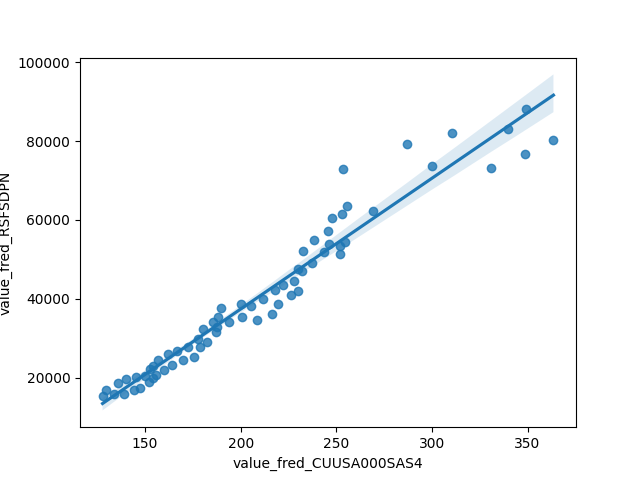
\includegraphics[scale = 0.9]{plots/plot_2026-11-18.png}
\caption{Raw Regression Plot for 2026-11-18}
\end{figure}
\newpage
\subsection{Detrended Regression}
\noindent Regresses the residuals of each series after removing its own linear time trend, so a shared trend can no longer drive the result on its own. A relationship that stays significant here is better evidence of a genuine link between the two series.

\begin{center}
\begin{tabular}{lclc}
\toprule
\textbf{Dep. Variable:}                       & value\_fred\_RSFSDPN\_detrended & \textbf{  R-squared:         } &     0.466   \\
\textbf{Model:}                               &               OLS               & \textbf{  Adj. R-squared:    } &     0.458   \\
\textbf{Method:}                              &          Least Squares          & \textbf{  F-statistic:       } &     58.51   \\
\textbf{Date:}                                &         Wed, 18 Nov 2026        & \textbf{  Prob (F-statistic):} &  1.03e-10   \\
\textbf{Time:}                                &             19:41:43            & \textbf{  Log-Likelihood:    } &   -672.47   \\
\textbf{No. Observations:}                    &                  69             & \textbf{  AIC:               } &     1349.   \\
\textbf{Df Residuals:}                        &                  67             & \textbf{  BIC:               } &     1353.   \\
\textbf{Df Model:}                            &                   1             & \textbf{                     } &             \\
\textbf{Covariance Type:}                     &            nonrobust            & \textbf{                     } &             \\
\bottomrule
\end{tabular}
\begin{tabular}{lcccccc}
                                              & \textbf{coef} & \textbf{std err} & \textbf{t} & \textbf{P$> |$t$|$} & \textbf{[0.025} & \textbf{0.975]}  \\
\midrule
\textbf{const}                                &    4.883e-10  &      505.070     &  9.67e-13  &         1.000        &    -1008.123    &     1008.123     \\
\textbf{value\_fred\_CUUSA000SAS4\_detrended} &     233.4966  &       30.526     &     7.649  &         0.000        &      172.566    &      294.427     \\
\bottomrule
\end{tabular}
\begin{tabular}{lclc}
\textbf{Omnibus:}       & 14.549 & \textbf{  Durbin-Watson:     } &    2.062  \\
\textbf{Prob(Omnibus):} &  0.001 & \textbf{  Jarque-Bera (JB):  } &   18.040  \\
\textbf{Skew:}          &  0.910 & \textbf{  Prob(JB):          } & 0.000121  \\
\textbf{Kurtosis:}      &  4.721 & \textbf{  Cond. No.          } &     16.5  \\
\bottomrule
\end{tabular}
%\caption{OLS Regression Results}
\end{center}

Notes: \newline
 [1] Standard Errors assume that the covariance matrix of the errors is correctly specified.

\begin{figure}
\centering
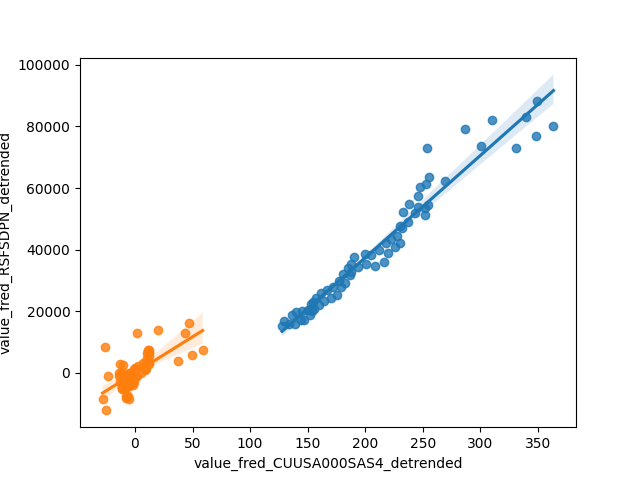
\includegraphics[scale = 0.9]{plots/plot_2026-11-18_detrended.png}
\caption{Detrended Regression Plot for 2026-11-18}
\end{figure}
\newpage
